\title{Statistical learning notes}
\author{Guanqun Cao\\
\texttt{guanqun.cao@tut.fi}}
\date{\today}
\documentclass[11pt, a4paper]{article}
\usepackage{graphicx,amssymb,amstext,amsmath}
\usepackage{color}
\usepackage{xcolor}
\usepackage{hyperref}
\usepackage{amsmath}
\usepackage{setspace}
\usepackage{fancyhdr}
\usepackage{fullpage}
%\usepackage{makeidx}
%\makeindex
\newif\ifarial
%\arialtrue
\arialfalse
\ifarial
\usepackage{helvet}
\renewcommand{\familydefault}{\sfdefault}% use arial font
\else
\usepackage{pslatex} % Times New Roman
\fi
\hypersetup{colorlinks=true, linkcolor=blue!50!black}
\begin{document}
\graphicspath{{"/home/cao/Dropbox/thesis/Documents/Notes/statlearning/img/"}}
\maketitle
\pagestyle{plain}
\section{Introducton}
Before going into the data analysis, try to visualize it to have a first impression.\\
Difference between machine learning and statistical learning:
\begin{itemize}
\item Machine learning has a greater emphasis on \emph{large scale} applications and \emph{prediction accuracy}.
\item Statistical learning emphasizes \emph{models} and their interpretability, and \emph{precision} and \emph{uncertainty}.
\end{itemize}
The supervised learning problem: 
\begin{itemize}
  \item Outcome meansure $Y$ also called dependent variable, reponse, target.
  \item Vector of $p$ predictor measurements $X$ also called inputs, regressors, covariates, features, independent variables.
  \item In the \emph{regression problem}, $Y$ is quantitative (e.g. price, blood pressure).
  \item In the \emph{classification problem}, $Y$ takes values in a finite, unordered set.
  \item We have training data. These are observations of these measurements.
  \end{itemize}
  On the basis of the training data we would like to 
  \begin{itemize}
    \item Accurately predict unseen test cases.
    \item Understand which inputs affect the outcome and how
    \item Assess the quality of our predictions and inferences.
    \end{itemize}
To apply supervised learning, one has to understand the simple methods first, in order to grasp the more sophsiticated ones. It is important to accurately assess the performance of a method, to know how well or how badly it is working.\par
In unsupervised learning,
\begin{itemize}
  \item No output/dependent variable (response), just a set of predictors (features) measured on a set of samples.
  \item objective is more fuzzy --- find groups of samples that behave similarly, find features that behave similarly, find linear combinations of features with teh most variation.
  \item difficult to evaluate the method.
  \item can be used as a pre-processing step for supervised learning.
\end{itemize}
We denote the input vector as 
\[
  X = \begin{pmatrix} 
    X_1\\ X_2 \\ X_3 \end{pmatrix},
\]
where $X$ refers to the variable and $x$ denotes as the instance, and we usually take column vectors.\\
The ideal $f(x)=E(Y|X=x)$ is called the regression function. 
\begin{itemize}
  \item The regression function $\hat{f}(x)$ is the ideal or optimal predictor of $Y$ with regard to mean-squared predictor of $Y$ with regard to mean-squared prediction error: $f(x)=E(Y|X=x)$ is the function taht minimize $E[(Y-g(X))^2|X=x]$ over all functions $g$ at all points $X=x$.
  \item We also have $\epsilon=Y-f(x)$ as the irreducible error.
  \item For any estimate $\hat{f}(x)$ of $f(x)$, we have
\[
  E[(Y-\hat{f}(X))^2|X=x]=[f(x)-\hat{f}(x)]^2+\operatorname{Var}(\epsilon).
\]
\item We relax the definition and let
  \[
    \hat{f}(x)=\operatorname{Ave}(Y|X\in \mathrm{N}(x)),
  \]
  where $\mathrm{N}(x)$ is some \emph{neighborhood} of $x$.
\item Nearest neighbor average can be pretty good for small number of components $p$, i.e. $p\leq 4$ and large $N$.
\item Nearest neighbors tend to far away in high dimensions. (Curse of dimensionality). Note the curve about the curse of dimensionality. NN is to have the average estimate whose variance is $10\%$ lower than the original data. A $10\%$ neighborhood in high dimensions need no longer be local, so we cannot estimate $E(Y|X=x)$ by local averaging. 
\end{itemize}
Some trade-offs:
\begin{itemize}
\item Prediction accuracy versus interpretability
\item Good fit versus over-fit or under-fit
\item Parsimony versus black-box
\end{itemize}
\begin{figure}
[h!]
\centering
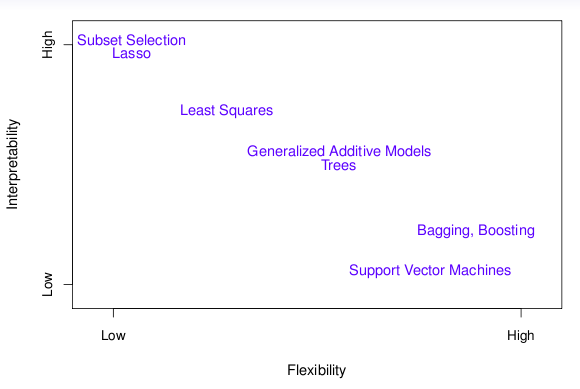
\includegraphics[width=.6\textwidth]{flex_vs_inter.png}
\caption{Interpretability vs flexibility.}
\end{figure}
We also have the Bias-Variance Trade-Off: The expected test MSE is
\[
  E(y_0-\hat{f}(x_0))^2=\operatorname{Var}(\hat{f}(x_0))+[\operatorname{Bias}(\hat{f}(x_0))]^2+\operatorname{Var}(\epsilon).
\]
\begin{itemize}
  \item The variance of a statistical learning method refers to the amount by which $\hat{f}$ would change if we estimated it using a different training dataset. In general, more flexible methods have higher variance.
  \item The Bias refers to the error that is introduced by approximating a real-life problem, which may be extremely complicated, by a much simpler model.
  \item As a general rule, as we use more flexible methods, the variance will increase and the bias will decrease. The relative rate of change of these two quantities determines whether the test MSE increases or decreases. 
\end{itemize}
For classification, the Bayes optimal classifier at $x$ is 
\[
  C(x)=j \text{ if } p_j(x)=\max\{p_1(x),p_2(x),\dots,p_K(x)\},
\]
where the conditional class probabilities at $x$ is
\[
  p_k(x)=\operatorname{Pr}(Y=k|X=x), k=1,2,\dots,K.
\]
\begin{itemize}
  \item The performance of $\hat{C}(x)$ using the misclassification error rate is:
    \[
      {\operatorname{Err}}_{\text{\textbf{Te}}}=\underset{i\in \text{\textbf{Te}}}{\operatorname{Ave}}\;I[y_i\neq \hat{C}(x_i)].
    \]
\end{itemize}
For K-nearest neighbor, increasing K will reduce the training error continuously, but test error first drops and then rises.
\section{Linear Regression}
\textbf{Linear regression} is a simple approach to supervised learning. It assumes that the dependence of $Y$ on $X_1,X_2,\dots,Xp$ is linear.\\
We assume a model
\[
Y=\beta_0+\beta_1 X + \epsilon,
\]
where $\beta_0$ and $\beta_1$ are two unknown constants that represent the intercept and slope, also known as \emph{coefficients} or \emph{parameters}, and $\epsilon$ is the error term.
Given some estiamtes $\hat{\beta}_0$ and $\hat{\beta}_1$ for the model coefficients, we have the prediction
\[
  \hat{y}=\hat{\beta}_0+\hat{\beta}_1 x,
\]
where $\hat{y}$ indicates a prediction of $Y$ on the basis of $X=x$.\\
Estimation of the parameters by least squares
\begin{itemize}
\item We define $e_i=y_i-\hat{y}_i$ as the $i$th \emph{residual}, Then the \emph{rsidual sum of squares} (RSS) is defined as
\begin{align}
\operatorname(RSS)&=e^2_1+e^2_2+\dots+e^2_n,\\
&=(y_1-\hat{\beta}_0-\hat{\beta}_1x_1)^2+(y_2-\hat{\beta}_0-\hat{\beta}_1x_2)^2+\dots+(y_n-\hat{\beta}_0-\hat{\beta}_1x_n)^2.
\end{align}
\item The least squares approach chooses $\hat{\beta}_0$ and $\hat{\beta}_1$ to minimize the $\operatorname{RSS}$. The minimizing values are 
  \begin{align}
  \hat{\beta}_0&=\bar{y}-\hat{\beta}_1 \bar{x},\\
    \hat{\beta}_1&=\frac{\sum_{i=1}^n(x_i-\bar{x})(y_i-\bar{y})}{\sum_{i=1}^n(x_i-\bar{x})^2},
  \end{align}
\end{itemize}
where $\bar{y}={1\over n}\sum_{i=1}^n y_i$ and $\bar{x}={1\over n}\sum_{i=1}^n x_i$ are the sample means.\\
Assessing the accuracy of the coefficient estimates.\\
Suppose we have random sample $x_1,x_2,\dots,x_n$. The standard error of the mean (SEM) is the standard deviation of the sample-mean's estimate of a population mean.
\[
  \operatorname{SE}_{\bar{x}}=\frac{s}{\sqrt{n}}
\]
where $s$ is the sample standard deviation and $n$ is the number of observations of the sample.\\
This estimate can be cmopared with the formula for the true standard deviation of the sample mean as $T/n$ as $T=(x_1,x_2,\dots,x_n)$:
\[
  \operatorname{SD}_{\bar{x}}=\frac{\sigma}{\sqrt{n}}.
\]
The standard errors associated with $\hat{\beta}_0$ and $\hat{\beta}_1$ are
\[
  \operatorname{SE}(\hat{\beta}_1)^2=\frac{\sigma^2}{\sum_{i=1}^n(x_i-\bar{x})^2}
\]
\[
  \operatorname{SE}(\hat{\beta}_0)^2 =\sigma^2[\frac{1}{n}+\frac{\bar{x}^2}{\sum_{i=1}^n(x_i-\bar{x})^2}]
\]
\textbf{Confidence interval}:\\
A $95\%$ confidence interval is defined as a range of values such that $95\%$ probability, the range will contain the true unknown value of the parameter, i.e. $\hat{\beta}_1\pm 2\cdot \operatorname{SE}(\hat{\beta}_1)$. This is a frequentist idea.\\[1mm]
\textbf{Standard errors} can also be used to perform hypothesis tests on the coefficients. 
\begin{itemize}
\item To test the null hypothesis, we compute a \emph{t-statistic}, given by
\[
  t=\frac{\hat{\beta}_1-0}{\operatorname{SE}(\hat{\beta}_1)},
\]
It measures the number of standard deviations that $\beta_1$ is away from 0.
\item This will have a $t$-distribution with $n-2$ degrees of freedom, assuming $\beta_1=0$.
\item Using statistical tools, we can compute the probability of observing any value equal to $|t|$ or larger. We call this probability the \emph{p-value}.
\item We interpret the p-value as follows: with a small p-value 
we can infer there is an association between the predictor and the response.
\end{itemize}
\textbf{Degree of freedom:} 
\begin{itemize}
\item In statistics, the number of degrees of freedom is the number of values in the final calculation of a statistic that are free to vary. It is the number of independent observations in a sample of data that are available to estimate a parameter of the population from which that sample is drawn. 
\item In general, the degrees of freedom of an estimate of a parameter are equal to the number of independent scores that go into the estimate minus the number of parameters used as intermediate steps in the estimation of the parameter itself, e.g.  the sample variance has N-1 degrees of freedom, since it is computed from N random scores minus the only 1 parameter estimated as intermediate step, which is the sample mean.
\end{itemize}
Assessing the overal accuracy of the model
\begin{itemize}
  \item We comptue the \emph{Residual Standard Error}
    \[
      \operatorname{RSE}=\sqrt{{1 \over n- 2} \operatorname{RSS}}=\sqrt{ {1 \over n-2} \sum_{i=1}^n (y_i-\hat{y}_i)^2},
    \]
    where the residual sum-of-squares is $\operatorname{RSS}=\sum_{i=1}^n (y_i-\hat{y}_i)^2$.
  \item \emph{R-squared} or fraction of variance explained is 
    \[
      R^2={\operatorname{TSS}-\operatorname{RSS} \over \operatorname{TSS} }=1-{\operatorname{RSS}\over\operatorname{TSS}}.
    \]
    where $\operatorname{TSS}=\sum_{i=1}^n (y_i-\bar{y}_i)^2$ is the total sum of squares.\\
$R^2$ is easier to interprete than RSE as it is between 0 and 1, but sometimes hard to determine what is a good $R^2$ value.
\item The $R^2$ statistic is the correlation between the two variables and measures how closely the input variable and the output variable are related. The $p$ value and $t$ statistic merely measure how strong is the evidence that there is a nonzero association. Even a weak effect can be extremely significant given enough data.\\[1mm] 
\end{itemize}
\textbf{Multiple Linear Regression}:\\[1mm]
It refers to regression models wth more than one predictor.
\begin{itemize}
\item Model: $Y=\beta_0+\beta_1 X_1 + \beta_2 X_2 + \beta_3 X_3$
\item we interpret $\beta_j$ as the \emph{average} effect on $Y$ of a one unit increase in $X_j$, holding all other predictors fixed.
\end{itemize}
Interpreting regression coefficients
\begin{itemize}
\item The ideal scenario is when the predictors are uncorrelated:
\begin{itemize}
\item Each coefficient can be estimated and tested separately
\item We can have the response depend on one predictors, with others fixed. 
\end{itemize}
\item The variance of all coefficients tends to increase, sometimes dramatically
\item Interpretations become hazadous
\item Claims of causality should be avoided for observational data.
\end{itemize}
Estimation and Prediction for Multiple Regression
\begin{itemize}
  \item Given estimates $\hat{\beta}_0, \hat{\beta}_1,\dots,\hat{\beta}_p$, we can make predictions using the formula 
\[
  \hat{y}=\hat{\beta}_0+\hat{\beta}_1x_1 + \hat{\beta}_2x2+\cdots+\hat{\beta}_px_p
\]
\item The sum of squared residuals is
  \begin{align}
    \operatorname{RSS}&=\sum_{i=1}^n(y_i-\hat{y}_i)^2\\
    &=\sum_{i=1}^n(y_i-\hat{\beta}_0-\hat{\beta}_1x_{i1}-\hat{\beta}_2x_{i2}-\cdots-\hat{\beta}_px_{ip})^2.
  \end{align}
  The values $\hat{\beta}_0,\hat{\beta}_1,\dots,\hat{\beta}_p$ minimize RSS are the multiple least squares regression coefficient estimates.
\end{itemize}
We define F-statistics
\[
  F=\frac{(\operatorname{TSS}-\operatorname{RSS}/p)}{\operatorname{RSS}/(n-p-1)}\sim F_{p,n-p-1}.
\]
\begin{itemize}
  \item If F-statistics is far larger than 1, it shows it is against the null hypothesis $H_0$.
  \item If F-statistic is significant, then we have extremely strong
    evidence that at least one of the predictors is associated with response.
\item If $n$ is large, an F-statistic that is just a little larger than 1 might still provide evidence against $H_0$, and vice versa.
\item When $H_0$ is true and the errors $\epsilon_i$ have a normal distribution, the F-statistic follows an F-distribution.
\item We can compute p-value from the F-statistic. And we can determine whether or not to reject $H_0$ based on the p-value.
\item There is a high chance to incorrectly conclude there is an association between the variable and the responce based on the individual t-statistics and associated p-values. The F-statistic does not suffer from this problem because it adjusts for the number of
  predictors.
\item If $p>n$ then there are more coefficients $\beta_j$ to estimate than observations from which to estimate them. We cannot fit the multiple linear regression model using least squares, so F-statistics cannot be used.
\end{itemize}
Deciding on the important variables
\begin{itemize}
  \item Forward selection: begin with the null model and add $p$ simple linear regressions that reults in the lowest RSS, until a stopping criterion is met.
  \item Backward selection: start with all variables in the model. Remove the one with the largest p-value iteratively, until a stopping criterion is met.
\end{itemize}
Qualitative Predictors
\begin{itemize}
\item They are discrete set of values.
\item Also called categorical predictors or factor variables.
\end{itemize}
Removing the additive assumption: \emph{interactions} and \emph{nonlinearity}.
\begin{itemize}
\item One input variable can influence another variable.
\item We can use the multiplication of the interacted variables to check the p-value of coefficent. It p-value is low, it indicates a strong interaction. 
\end{itemize}
Polynomial regression is the linear regression with non-linear regression functions.\\[1mm]
The hierarchy principle: If we include an interaction in a model, we should also include the main effects, even if the p-values assocated with their coefficients are not significant.\\
We can also have linear coefficients but non-linear functions of variable.\\[1mm]
Outliers\\[1mm]
Non-constant variance of error terms\\[1mm]
High leverage points\\[1mm]
Collinearity\\[1mm]
Statistical variability\\[1mm]
Scatter plot and box plot are two most common data visualization methods. For box plot
\begin{itemize}
\item The bottom and top of the box are always the first and third quartiles, and the band inside the box is always the second quartile (the median). 
\item The very bottom and top line are the hinges, which are the ranges.
\end{itemize}
\section{Classification}
We can use Linear Regression for binary classification problems, which is equivalent to \emph{linear discriminant analysis}. $E(Y|X=x)=\operatorname{Pr}(Y=1|X=x)$. But for multiclass problems, we cannot use linear regression.\\[1mm]
\subsection{Logistic Regression:}
We have $p(X)=\operatorname{Pr}(Y=1|X)$ and it has the form
\[
  p(X)=\frac{e^{\beta_0+\beta_1X}}{1+e^{\beta_0+\beta_1X}}
\]
$p(X)\in [0,1]$.\\
We also have the \emph{log odds} or \emph{logit transformation} of $p(X)$ as
\[
  \log(\frac{p(X)}{1-p(X)})=\beta_0+\beta_1 X.
\]
We use maximium likelihood to estimate the parameters.
\[
  \ell(\beta_0,\beta)=\prod_{i:y_i=1}p(x_i)\prod_{i:y_i=0}(1-p(x_i)).
\]
The likelihood gives the probabilitiy of the observed zeros and oens in the data. We pick $\beta_0$ and $\beta_1$ to maximize the likelihood of the observed data.\\[1mm]
Logistic regression with several variables
\[
  \log(\frac{p(X)}{1-p(X)})=\beta_0+\beta_1X_1+\dots+\beta_pX_p
\]
\[
  p(X)=\frac{e^{\beta_0+\beta_1X_1+\dots+\beta_pX_p}}{1+e^{\beta_0+\beta_1X_1+\dots+\beta_pX_p}}.
\]
Confounding\\
Scatter plot: a type of mathematical diagram using Cartesian coordinates to display values for typically two variables for a set of data. If the points are color-coded you can increase the number of displayed variables to three.\\[1mm]
Tilde in R:\\
The thing on the right of $\leftarrow$ is a formula object. It is often used to denote a statistical model, where the thing on the left of the $\sim$ is the response and the things on the right of the $\sim$ are the explanatory variables. So in English you'd say something like ``Species depends on Sepal Length, Sepal Width, Petal Length and Petal Width''.\\
Data Frame: The concept of a data frame comes from the world of statistical software used in empirical research; it generally refers to ``tabular'' data: a data structure representing cases (rows), each of which consists of a number of observations or measurements (columns). Alternatively, each row may be treated as a single observation of multiple ``variables''. In any case, each row and each column has the same data type, but the row (``record'') datatype may be heterogenous (a tuple of different types), while the column datatype must be homogenous. Data frames usually contain some metadata in addition to data; for example, column and row names.\\[1mm]
Case-control sampling and logistic regression
\begin{itemize}
  \item With case-control samples, we can estimate the regression parameters $\beta_j$ accurately if our model is correct, the constant term $\beta_0$ is incorrect.
  \item We can correct the estimated intercept by a simple transformation
  \[
    \hat{\beta}_0^*=\hat{\beta}_0+\log{\frac{\pi}{1-\pi}}-\log{\frac{\tilde{\pi}}{1-\tilde{\pi}}},
  \]
  where $\pi$ is the true probability and $\tilde{\pi}$ is the case probability.
  \item Often cases are rare and we take them all; up to five times that number of controls is sufficient.
  \item Case/Control sampling is most effective when the prior probabilities of the classes are very unequal. We expect this to be the case for the cancer and spam problems, but not the gender problem.
\end{itemize}
Logistic regression with more than two classes
\begin{itemize}
  \item One version used in R package \emph{glmnet} (Softmax function). It has the symmetric from
  \[
    \operatorname{Pr}(Y=k|X)=\frac{e^{\beta_{0k}+\beta_{1k}X_1+\dots+\beta_{pk}X_p}}{\sum_{\ell=1}^Ke^{\beta_{0\ell}+\beta_{1\ell}X_1+\dots+\beta_{p\ell}X_p}},
  \]
  where $K$ is the number of classes, and $K>2$. Each class has a linear function, and we weight against each other using an exponential function.
\item It is also referred to as multinomial regression.
\end{itemize}
\subsection{Discriminant Analysis}
\begin{itemize}
  \item It models the distribution of $X$ in each of the classes separately, and then use \emph{Bayes theorem} to flip things around and obtain $\operatorname{Pr}(Y|X)$.
  \item When we use normal distributions for each class, it leads to linear or quadratic discriminant analysis.
  \item It is quite generic, and applies to other distributions as well.
\end{itemize}
Bayes theorem for classification
From the Bayes theorem, 
\[
\operatorname{Pr}(Y=k|X=x)=\frac{\operatorname{Pr}(X=x|Y=k)\cdot\operatorname{Pr}(Y=k)}{\operatorname{Pr}(X=x)},
\]
Or
\[
P(Y \mid X) = \frac{P(X \mid Y)}{\sum_i {P(X \mid Y_i) P(Y_i)}} \cdot P(Y) 
\]
we can write the discriminant analysis as
\[
  \operatorname{Pr}(Y=k|X=x)=\frac{\pi_kf_k(x)}{\sum_{l=1}^K\pi_lf_l(x)},
\]
where $f_k(x)=\operatorname{Pr}(X=x|Y=k)$ is the density for $X$ in class $k$, and we use normal densities separately for each class. $\pi_k=\operatorname{Pr}(Y=k)$ is the marginal or \emph{prior} probability for class $k$.\\[1mm]
Comparison between Logistic Regression and Discriminant Analysis
\begin{itemize}
  \item When the classes are well-separated, the parameter estimates for the logistic regression model are unstable. Linear Disciminant Analysis (LDA) does not suffer from this problem.
  \item If $n$ is small and the distribution of the predictors $X$ is approximately normal in each of the classes, LDA is more stable.
  \item LDA is popular when we have more than two classes, because is also provides low-dimensional views of the data.
\end{itemize}
Linear Discriminant Analysis when $p=1$\\
\[
f_k(x) \sim \mathcal{N}(\mu_k,\,\sigma_k^2),
\]
where $\mu_k$ and $\sigma_k^2$ are the mean and variance of class $k$ respectively, and we assume all $\sigma_k=\sigma$ are the same.\\
We can plug in the former equation into the bayes formula. and perform some cancellation and simplification. To classify $X=x$, we need to find the largest $p_k(x)$. Taking logs, and discarding terms that do not depend on $k$, we see that it is equivalent to assigning $x$ to the class with the largest \emph{discriminant score}:
\[
  \delta_k(x)=x\cdot \frac{\mu_k}{\sigma^2}-\frac{\mu_k^2}{\sigma^2}+\log(\pi_k).
\]
$\delta_k(x)$ is a \textbf{linear} function of $x$.
Parameter estimation
\begin{align}
  \hat{\pi}_k&=\frac{n_k}{n}\\
  \hat{\mu}_k&= \frac{1}{n_k} \sum_{i:y_i=k}x_k\\
  \hat{\sigma}^2&=\frac{1}{n-K} \sum_{k=1}^K \sum_{i:y_i=k}(x_i-\hat{\mu}_k)^2\\
 &=\sum_{k=1}^K\frac{n_k-1}{n-K}\cdot \hat{\sigma}_k^2.
\end{align}
where $\hat{\sigma}^2_k=\frac{1}{n_k-1}\sum_{i:y_i=k}(x_i-\hat{\mu}_k)^2$ is the usual formula for the estimated variance in the $k$th class.\\[1mm]
Linear Discriminant Analysis when $p>1$\\
Density: 
\[f(x)=\frac{1}{(2\pi)^{p/2}|\Sigma|^{1/2}}e^{-{1\over 2}(x-\mu)^\top\Sigma^{-1}(x-\mu)}.
\]
Discriminant function:
\[
  \delta_k(x)=x^\top\Sigma^{-1}\mu_k-{1\over 2}\mu_k^T\Sigma^{-1}\mu_k+\log\pi_k.
\]
but it remains linear.\\
Fisher's Disciminant Plot:\\
When there are $K$ classes, linear discriminant analysis can be viewed in a $K-1$ dimensional plot. It classifies to the closest centroid, and they span a $K-1$ dimensional plane.\\[1mm]
Probabilisitic interpretation\\
Once we have estimates $\hat{\delta_k}(x)$, we can turn these functions into estimates for class probabilities:
\[
 \hat{\operatorname{Pr}}(Y=k|X=x)=\frac{e^{\hat{\delta}_k(x)}}{\sum_{l=1}^Ke^{\hat{\delta}_l(x)}}.
\]
The ROC curve shows true positive rate and false positive rate simultaneously. The curve traces out when changing the threshold. We also use the AUC or area under the curve to compare the performance between classifiers with different thresholds. Higher AUC is good.\\[1mm]
Other forms of Discriminant Analysis\\
\[
  \operatorname{Pr}(Y=k|X=x)=\frac{\pi_kf_k(x)}{\sum^K_{l=1}\pi_lf_l(x)}
\]
When $f_k(x)$ are Gaussian densities, with the same covariance matrix $\Sigma$ in each class, it leads to LDA. By altering the forms for $f_k(x)$, we get different classifiers as
\begin{itemize}
  \item With Gaussians but different $\Sigma_k$ in each class, we get quadratic discriminant analysis.
  \item With $f_k(x)=\prod^p_{j=1}f_{jk}(x_j)$ (conditional independence model) in each class we get naive Bayes. For Gaussian this means the $\Sigma_k$ are diagonal.
  \item Many other forms, by proposing specific density models for $f_k(x)$, including nonparametric approaches.
  \end{itemize}
  Quadratic Discriminant Analysis
  \[
    \delta_k(x)=-{1\over2}(x-\mu_k)^\top \Sigma_k^{-1}(x-\mu_k)+\log\pi_k-{1\over2}\log|\Sigma_k|
  \]
  The quandratic terms matter as $\Sigma_k$ are different.\\[1mm]
Naive Bayes\\
Assume features are independent in each class. NB is Useful when $p$ is large, and multiviariate methods like QDA and even LDA break down due to large covariance matrices.
\begin{itemize}
  \item Gaussian naive Baye assumes each $\Sigma_k$ is diagonal:
    \begin{align}
    \delta_k(x) & \sim \log\bigg[\pi_k\prod_{j=1}^pf_{ij}(x_j)\bigg]\\
    & = -{1\over2}\sum_{j=1}^p\bigg[\frac{(x_j-\mu_{kj})^2}{\sigma^2_{kj}}+\log\sigma^2_{kj}\bigg]+\log\pi_k.
  \end{align}
\item can use for mixed feature vectors (qualitative and quantitative). If $X_j$ is qualitative, replace $f_{kj}(X_j)$ with probability mass function (histogram) over discrete categories.
\end{itemize}
Compare Logistic Regression and LDA\\
For a two-class problem, one can show for LDA
\[
  \log\bigg({p_1(x)\over{1-p_1(x)}}\bigg)=\log\bigg(\frac{p_1(x)}{p_2(x)}\bigg)=c_0+c_1x_1+\dots+c_px_p.
\]
It has the same form as logistic regression. The difference is in how the parameters are estimated.
\begin{itemize}
  \item Logistic regression uses the conditional likelihood based on $\operatorname{Pr}(Y|X)$, known as discriminative learning.
  \item LDA uses the full likelihood based on $\operatorname{Pr}(X,Y)$, known as generative learning.
  \item Despite these differences, in practice the results are often very similar.
\end{itemize}
\section{Resampling}
Validation method: We split the original training set into a train and validation set. Then, we fit models of various set sizes and of various model sizes. Our job is to find $\hat{k}$, and return the model $\mathcal{M}_{\hat{k}}$.
\begin{itemize}
  \item two major methods: cross validation and the bootstrap
  \item Resampling refits a model of interest to samples formed from the training set, in order to obtain addtional information about the fitted model.
  \item They provide estimates of test set prediction error, and the standard deviation and bias of our parameter estimates.
  \end{itemize}
Drawbacks of validation set approach
\begin{itemize}
\item the validation estimate of the test error can be highly variable, depending on precisely which observations are included in the training set and which observations are included in the validation set
\item Only a subset of the observation are used for training
\item The validation set error may tend to overestimate the test error for the model fit on the entire dataset. 
\end{itemize}
K-fold cross validation
\begin{itemize}
\item random divides the data into $K$ equal-size parts. We leave out. We leave out part $k$, fit the model to the other $K-1$ parts (combined), and then obtain predictions for the left-out $k$th part.
\item Let the $K$ parts be $C_1,C_2,\dots C_K$ where $C_k$ denotes the indices of the observations in part $k$. There are $n_k$ observations in part $k$: if $N$ is a multiple of $K$, then $n_k=n/K$.
\item Computer
  \[
    CV_{(K)}=\sum_{k=1}^K{n_k\over n}\operatorname{MSE}_k,
  \]
  where $\operatorname{MSE}_k\sum_{i\in C_k}(y_i-\hat{y}_i)^2/n_k$ and $\hat{y}_i$ is the fit for observation $i$, obtained from the data with part $k$ removed.
\item Setting $K=n$ yield $n$-fold or leave-one out cross validation.
\end{itemize}
Leave-one-out cross validation
\begin{itemize}
  \item With least squares linear or polynomial regression, an amazing shortcut maeks the cost of leave-one out cross validation the same as that of a single model fit. 
\[
  \operatorname{CV}_{(n)}={1\over n}\sum_{i=1}^n\bigg(\frac{y_i-\hat{y}_i}{1-h_i}\bigg)^2.
\]
where $\hat{y}_i$ is the $i$the fitted value from the original least squares fit, and $h_i$ is the leverage. It is like the ordinary MSR, except the $i$the residual is divided by $1-h_i$.
\item It does not shake up the data enough. The estimates from each fold are highly correlated and hence their average can have high variance.
\item $K=5, 10$ is a better choice.
\end{itemize}
  Problems with Cross validation
\begin{itemize}
\item Since each training set is only $(K-1)/K$ as big as the original training set, the estimates of prediction error will typically be biased upward.
\item The biase is minimized when $K=n$ (leave one out), the estimae has high variance.
\item $K=5 \text{or} 10$ provides a better compromise.
\end{itemize}
Cross Validation for Classification
\begin{itemize}
\item Compute
  \[
    CV_K=\sum_{k=1}^K{n_k\over n}\operatorname{Err}_k
  \]
  where $\operatorname{Err}_k=\sum_{i\in C_k}I(y_i\neq \hat{y}_i)/n_k$.
\item The estimated standard deviation of $\operatorname{CV}_k$ is 
\[
  \hat{\operatorname{SE}}(CV_k)=\sqrt{\sum_{k=1}^K\operatorname{Err}_k-\bar{\operatorname{Err}_k}^2/(K-1)}.
\]
\end{itemize}
Cross validation: right and wrong
\begin{itemize}
\item If we pre-select the predictors correlated to the class labels, we should not ignore this fact when applying cross validation. The procedure has already seen the labels of the training data and made use of them. It is a form of training and should be included in the validation process.
\item The right way is to apply screening and validation at each round of cross validation.
\end{itemize}
The bootstrap
\begin{itemize}
  \item For real data, we cannot generate new samples from the original population.
  \item Bootstrap allows to use computer to mimic the processing of obtaining new data sets, so that we can estimate the variability of our estimate without generating additonal samples.
  \item Rather than repeatedly obtaining independent datasets from the population, we obtain distinct datasets by repeatedly sampling obserations from the original dataset with \emph{replacement}.
  \item The procedure is repeated $B$ times for some large value of $B$, in order to produce $B$ different bootstrap datasets, $Z^{*1},Z^{*2},\dots Z^{*B}$ and $B$ corresponding $\alpha$ estimates, $\hat{\alpha}^{*1},\hat{\alpha}^{*2}\dots \hat{\alpha}^{*B}$.
  \item We estimate the standard error of these bootstrap estimates using the formula
\[
  \operatorname{SE}_B(\hat{\alpha})=\sqrt{{1\over {B-1}}\sum_{r=1}^B(\hat{\alpha}^{*r}-\bar{\hat{\alpha}}^*)^2}
\]
\end{itemize}
\begin{figure}
[h!]
\centering
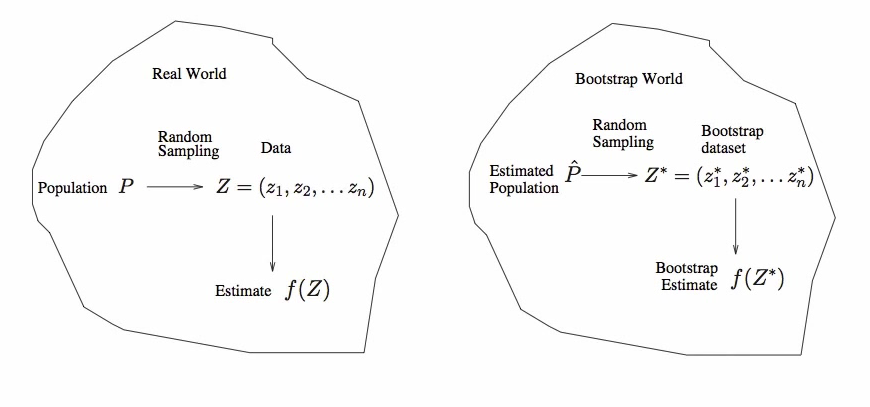
\includegraphics[width=.8\textwidth]{bootstrap.png}
\caption{Sampling and resampling.}
\end{figure}
\begin{itemize}
  \item In time series data, where data is not iid., we cannot bootstrap the data with replacement, but we can apply block boostrap.
  \item Primarily used to obtain standard erros of an estimate
\item also provides approximate confidence intervals for a population parameter, which represents an approximate $90\%$ confidence intervial for the true $\alpha$.
\item The above interval is called a \emph{Bootstrap Percentile} confidence interval. It is the simplest method for obtain a confidence interval from the bootstrap.
\end{itemize}
Compare Bootstrap and Cross Validation
\begin{itemize}
\item In CV, there is no overlap
\item To estimate prediction error using the bootstrap, we could think about using each bootstrap dataset as our training sample, and the original samples as our validation set.
\item But each bootstrap sample has significant overlap with the original data. About two-thirds of the original data points appear in each bootstrap sample. 
\end{itemize}
\section{Linear Model Selection and Regularization}
\subsection{Subset selection}
The reason to alternate Least Square methods
\begin{itemize}
\item Prediction Accuracy: when $p>n,$, to control the variance.
\item Model Interpretability: By setting the corresponding coefficient estimates to zero --- we can obtain a model that is more easily interpreted. Feature selection.
\end{itemize}
Three major classes of methods
\begin{itemize}
  \item \emph{Subset Selection}: We identify a subset of the $p$ predictors that we believe to be related to the response. We then fit the model using least squares on the reduced set of variables.
  \item \emph{Shrinkage:}: We fit a model involving all $p$ preditors, but the estimated coefficients are shrunken towards zero relative to the least squares estimates. The shrinkage aka regularization has the effect of reducing variance and can perform variable selection.
  \item \emph{Dimension Reduction}. We project the $p$ predictors into a $M$-dimensinoal subspace, where $M<p$. This is achieved by computing $M$ different linear combinations, or projections of the variables. Then these $M$ projections are used predictors to fit a linear regression model by least square. 
\end{itemize}
Best Subset Selection
\begin{enumerate}
\item Let $M_0$ denote the \emph{null model}, which contain no predictors. This model simply predicts the sample mean for each observation.
\item For $K=1,2,\dots p$:
\begin{enumerate}
\item Fit all $p \choose k$ models that contain exactly $k$ predictors.
\item Pick the best among these $p \choose k$ models, and call it $\mathcal{M}_k$. Choose the best model having the smallest RSS, or largest $R^2$.
\end{enumerate}
\item Select a single best frmo among $M_0,M_1,\dots,M_p$ using cross-validated prediction error, $C_p$ (AIC), (BIC), or adjusted $R^2$.
\end{enumerate}
Subset Selection applies to many methods, including least square regression, logistic regression, and so on. The deviance--- negative two times the maximized log-likelihood---plays the role of RSS for a broader class of models.\\[1mm]
Stepwise Selection
\begin{itemize}
\item Best subset selection does not apply with very large $p$. It leads to a large search space, and overfitting. And the complexity is $O(2^p)$.
\item Forward stepwise selection begins with a model containing no predictors, and then adds predictors to the model, one-at-a-time, until all of the predictors are in the model.
\item at each step the variable that gives the greatest additional improvement to the fit is added to the model.
\item Complexity: $O(p^2)$
\end{itemize}
The other around is Backward Stepwise Selection.
\begin{itemize}
  \item It searches through $1+p(p+1)/2$ models, same as forward subset selection.
  \item Backward selection requires the number of sample $n$ larger than the number of variables $p$, so that the full model can be fit. But forward does not have the requirement.
  \end{itemize}
  \subsection{Some criterions}
$C_p$, AIC, BIC and adjusted $R^2$
\begin{itemize}
  \item They adjust the training error for the model size, and can be used to select among a set of models with different number of variables.
  \item Mallow's $C_p$
    \[
      C_p={1\over n}(\operatorname{RSS}+2d\hat{\sigma}^2),
    \]
    where $d$ is the total number of parameters used and $\hat{sigma}^2$ is an estimate of the variance of the error $\epsilon$ associated with each response measurement. And $n>p$.
\item The AIC criterion is defined for a large class of models fit by maximum likelihood:
\[
\operatorname{AIC} = -2\log L+2\cdot d,
\]
where $L$ is the maximized value of the likelihood function for the estimated model.
\item In the case of the linear model with Gaussian errors, maximium likelihood and least squares are the equivalent. 
  \[
    -2\log L =\operatorname{RSS}/\hat{\sigma}^2
  \]
  \end{itemize}
  Bayesian Information Criterion (BIC)
\begin{itemize}
  \item $\operatorname{BIC}={1\over n}(\operatorname{RSS}+\log(n)d\hat{\sigma}^2).$
  \item Like $C_p$, the BIC will tend to take on a small value for a model with a low test error, and so generally we select the model that has the lowest BIC value.
  \item BIC replaces the $2d\hat{\sigma}^2$ used by $C_p$ with a $\log(n)d\hat{\sigma}^2$ term, where $n$ is the number of observations.
  \item Since $\log n > 2$ for any $n>7$, the BIC statistics generally places a heavier penalty on models with many variables, and hence results in the slection of smaller models than $C_p$.
\end{itemize}
Adjusted $R^2$
\begin{itemize}
\item For a least squares model with $d$ variables, the adjusted $R^2$ statistic is calculated as 
    \[
      \text{Adjusted }R^2=1-\frac{\operatorname{RSS}/(n-d-1)}{\operatorname{TSS}/(n-1)}.
    \]
    where TSS is the total sum of squares.
\item Unlike $C_p$, AIC, and BIC, for which a small value indicates a model with a low test error, a large value of adjusted $R^2$ indicateds a model with a small test error.
\item Maximizing the adjusted $R^2$ is equivalent to minimizing $\operatorname{RSS}/(n-d-1).$ While RSS always decreases as the number of variables in the model inceases, $\operatorname{RSS}/(n-d-1)$ may increase or decrease, due to the presence of $d$ in the denominator.
\item unlike the $R^2$ statistic, the adjusted $R^2$ statstic pays a price for the inclusion of unnecessary variables in the model.
\end{itemize}
Validation and Cross-Validation
\begin{itemize}
  \item The procedure has an adavantage over AIC, BIC, $C_p$ and adjusted $R^2$, in that it provides a direct estimate of the test error, and does not require an estimate of the error variance $\sigma^2$. 
  \item It can also be used in a wider range of model selection tasks, even in cases where it is hard to pinpoint the model degrees of freedom (the number of predictors in the model) or hard to estimate the error variance $\sigma^2$.
\end{itemize}
One-standard-error rule: We first calculate the standard error of the estimated test MSE for each model size, and the select the smallest model for which the estimated test error is within oen standard error of the lowest point on the curve.\\[1mm]
\subsection{Shrinkage Methods}
Ridge regression and Lasso
\begin{itemize}
\item The subset selection methods use least squares to fit a linear model that contains a subset of predictors.
\item Alternatively, we can fit a model containing all $p$ predictors using a technique that constrains and regularizes the coefficient estimates, or shrinks the coefficient estimates towards zero.
\item It may not be immediately obvious why such as contraint should improve the fit, but it turns out that shrinking the coefficient estimates can significantly reduce their variance.
\end{itemize}
Ridge Regression
\[
  \sum_{i=1}^n\bigg(y_i-\beta_0-\sum_{j=1}^p\beta_j x_{ij}\bigg)^2+\lambda\sum_{j=1}^p\beta_j^2=\operatorname{RSS}+\lambda\sum_{j=1}^p\beta_j^2,
\]
where $\lambda\geq 0$ is a tuning parameter, to be determined separately.\\[1mm]
\begin{itemize}
\item As with least squares, ridge regression seeks coefficient estimates that fit the data well, by making the RSS small.
\item However, the second term $\lambda\sum_j\beta_j^2$ called a shrinkage penalty, is small when $\beta_1,\dots,\beta_p$ are close to zero, and so it has the effect of shrinking the estimates of $\beta_j$ towards zero.
\item The tuning parameter $\lambda$ serves to control the relative impact of these two terms on the rgerssion coefficient estimates.
\item Selecting a good value for $\lambda$ is ciritical, cross validation is used for this.
  \end{itemize}
  Ridge Regression: scaling of predictors
\begin{itemize}
  \item The standard least squares coefficient estimates are scale equivariant: multiplying $X_j$ by a constant $c$ simply leads to a scaling of the least squares coefficient estimates by a factor of $1/c$. In other words, regardless of how the $j$th predictor is scaled, $X_j\hat{\beta}_j$ will remain the same.
  \item In contrast, the ridge regression coefficient estimates can change substantially when multiplying a given predictor by a constant, due to the sum of squared coefficients term in the penalty part of the ridge regression objective function.
  \item It is best to apply ridge regression after standardizing the predictors, using the formula
\[
\tilde{x}_{ij}=\frac{x_{ij}}{{1\over n}\sum_{i=1}^n(x_{ij}-\bar{x}_j)^2}
\]
\end{itemize}
One disadvantage of Ridge Regression is instead of involving a subset of variables in subset selection, ridge regression will include all $p$ predictors in the final model.\\
The Lasso is a relatively new alternative to ridge regression that overcomes the disadvantage. The lasso coefficients, $\hat{\beta}_\lambda^L$ minimize the quantity
\[
  \sum_{i=1}^n\bigg(y_i-\beta_0-\sum_{j=1}^p\beta_jx_{ij}\bigg)+\lambda\sum_{j=1}^p|\beta_j|=\operatorname{RSS}+\lambda\sum_{j=1}^p|\beta_j|.
\]
In statistical parlance, the lasso uses an $\ell_1$ penalty instead of an $\ell_2$ penalty. The $\ell_1$ norm of a coefficient vector $\beta$ is given by $\|\beta\|_1=\sum|\beta_j|$.
\begin{itemize}
\item As with ridge regression, the lasso shrinks the coefficients estimates towards zero.
\item In the case of lasso, the $\ell_1$ penalty ahs the effect of forcing some of the coefficient estimates to be exactly equal to zero when the tuning paramter $\lambda$ is suffciently large.
\item Much like best subset selection, the lass performs variable selection.
\item We say that the lasso yields sparse models --- that is models that involve only a subset of the variables.
\item As in ridge regression, selecting a good value of $\lambda$ for the lasso is critical; cross-validation is the method of choice.
\end{itemize}
\begin{figure}
[h!]
\centering
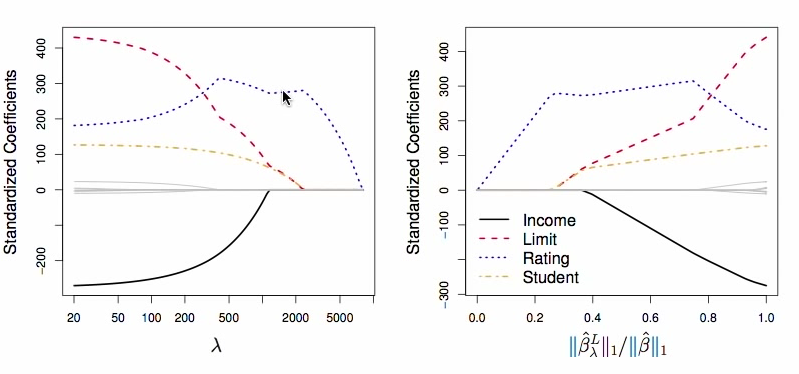
\includegraphics[width=.8\textwidth]{lasso.png}
\caption{Lasso shrinks several variables towards zero.}
\end{figure}
We can see from the graph that by increasing $\lambda$, we can shrink some variables to exactly zero.\\
The Variable Selection Property of the Lasso\\
Why is it that the lasso, unlike ridge regressio, results in coefficent estimates that are exactly equal to zero? It is equivalent to say the lasso and ridge regression coefficient estimates solve the problems
\begin{align}
  \min_\beta&\sum_{i=1}^n\bigg(y_i-\beta_0-\sum_{j=1}^p\beta_jx_{ij}\bigg)^2\\
  \text{ subject to }& \sum_{j=1}^p|\beta_j|\leq s.
\end{align}
and 
\begin{align}
  \min_\beta&\sum_{i=1}^n\bigg(y_i-\beta_0-\sum_{j=1}^p\beta_jx_{ij}\bigg)^2\\
  \text{ subject to }& \sum_{j=1}^p\beta_j^2\leq s.
\end{align}
\begin{figure}
[h!]
\centering
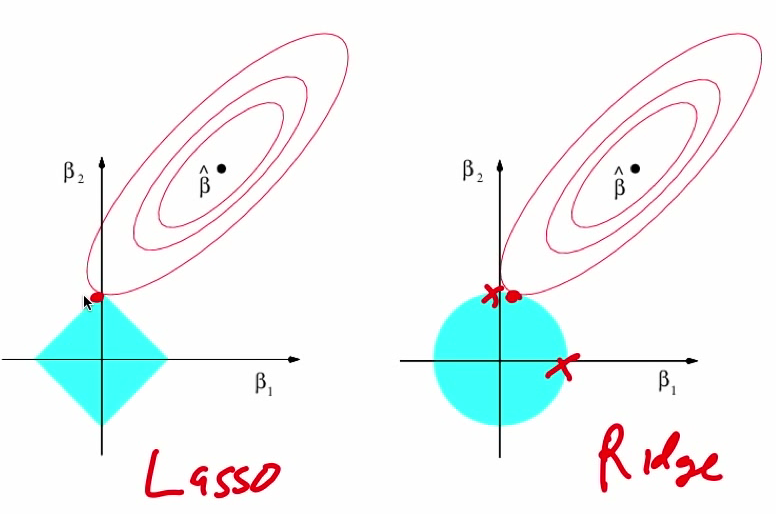
\includegraphics[width=.6\textwidth]{lasso_solution.png}
\caption{The lasso solution reaches the corner, which gives the sparsity.}
\end{figure}\\
Selecting the tuning parameter for ridge regression and lasso using cross validation\\
We choose a grid of $\lambda$ values, and compute the cross validation error rate for each value of $\lambda$. We then select the tuning parameter avlue for which the cross validation error is the smallest. $d\leq p$ but is unknown, so BIC, AIC and adjusted $R^2$ cannot be used.
\subsection{Dimension Reduction Methods}
\begin{itemize}
  \item Let $Z_1,Z_2,\dots,Z_M$ represent $M<p$ linear combinations of our original $p$ predictors. That is
\[
  Z_m=\sum_{j=1}^p\phi_{mj}X_j
\]
for some constants $\phi_{m1},\dots,\phi_{mp}$.
\item We can then fit the linear regression model
  \[
    y_i=\theta_0+\sum_{m=1}^M\theta_m z_{im}+\epsilon_i, i=1,\dots,n
  \]
using ordinary least squares.
\item Note that in the second mode, the regression coefficients are given by $\theta_0,\theta_1,\dots,\theta_M$. If the constants $\phi_{m1},\dots,\phi_{mp}$ are chosen wisely, the dimension reduction approaches can often outperform OLS regression.
\item We do the transform as
  \[
    \sum_{m=1}^M\theta_m z_{im}=\sum_{m=1}^M\theta_m\sum_{j=1}^p \phi_{mj}x_{ij}=\sum_{j=1}^p\sum_{m=1}^M\theta_m\phi_{mj}x_{ij}=\sum_{j=1}^p\beta_jx_{ij}
  \]
  where
  \[
    \beta_j=\sum_{m=1}^M\theta_m\phi_{mj}.
  \]
\item Dimension reduction serves to constrain the estimated coefficients, since now th ey must take the form as above.
\end{itemize}
Principal Component Regression
\begin{itemize}
  \item PCR identifies linear combations or direction that best represent the predictors $X_1,\dots,X_p$. 
  \item These directions are identifies in an unsupervised way, since the response $Y$ is not used to help determine th e principal component directions.
  \item The response does not supervise the identification of the principal component. 
  \item There is no guarantee that the directions represent the predictors are the bes t directions for predicting the response.
\end{itemize}
Partial Least Squares (PLS)
\begin{itemize}
\item Unlike PCR, PLS identifies the new features in a supervised manner --- it makes use of the response $Y$ in order to identify new featuers that not only approximate the old features well, but are related to the response.
\item Rougthly speaking, the PLS approach attempts to find directions that help explain both the response and the predictors.
\end{itemize}
PLS
\begin{itemize}
  \item After standardizing the $p$ predictors, PLS computes the first direction $Z$ by setting each $\phi_{1j}$ equal to the coefficient from the simple linear regression of $Y$ onto $X_j$.
  \item One can show this coefficient is proportional to the correlation between $Y$ and $X_j$.
  \item In computing $Z_1=\sum^p_{j=1}\phi_{1j}X_j$, PLS places the highest weight on the variables that are most strongly related to the response.
  \item Subsequent directions are found by taking residuals and then repeating the above prescription.
\end{itemize}
Polynomial Regression
\begin{itemize}
  \item \[
y_i=\beta_0+\beta_1x_i+\beta_2x_i^2+\beta_3x_i^3+\dots+\beta_3x_i^d+\epsilon_i
\]
\item We look into the fitted function values at any value $x_0$:
  \[
    \hat{f}(x_0)=\hat{\beta}_0+\hat{\beta}_1x_0+\hat{\beta}_2x_0^2+\dots+\hat{\beta}_kx_0^k
  \]
\item Since $\hat{f}(x_0)$ is a linear function of the $\hat{\beta}_\ell$, we can get simple expression for pointwise-variances $\operatorname{Var}[\hat{f}(x_0)]$ at any value $x_0$.
\item We either fix the degree $d$ at some reasonble low value, or use cross validation.
\item Nonlinear Logistic Regression
  \[
    P(Y>250|X=x_i) = \frac{\exp(\beta_0+\beta_1x_i+\beta_2x_i^2+\dots+\beta_dx_i^d)}{1+\exp(\beta_0+\beta_1x_i+\beta_2x_i^2+\dots+\beta_dx_i^d)}
  \]
\item To get confidence intervals, compute upper and lower bounds \emph{on the logit scale}, and then invert to get on probabiility scale.
\item Can do separately on several variables --- just stack the variables into one matrix, and separate out the pieces afterwards
\item Caveat: polynomials have notrious tail behavior -- very bad for extrapolation.
\end{itemize}
Step Functions\\
Another way of creating transformations of a variable --- cut the variable into distinct regions. It is a local model. It is easy to work with, which creates a series of dummy variables representing each group.\\[1mm]
Piecewise Polynomials
\begin{itemize}
\item Instead of a single polynomial in $X$ over its whole domain, we can rather use different polynomials in regions defined by knots.
  \[
    y_i= \begin{cases} 
      \beta_{01}+\beta_{11}x_i+\beta_{21}x_i^2+\beta_{31}x_i^3+\epsilon_i \text{ if }x_i<c; \\
      \beta_{02}+\beta_{12}x_i+\beta_{22}x_i^2+\beta_{32}x_i^3+\epsilon_i \text{ if }x_i<c; \\
    \end{cases} 
  \]
\item Better to add constraints to the polynomials, e.g. continuity
\item Splines have the ``maximum'' amount of continuity
\end{itemize}
\subsection{Nonline methods}
Linear Splines\\
A linear spline with knots at $\epsilon_k, k=1,\dots,K$ is a piecewise linear polynomial continuous at each knot.\\
We can represent this model as
\[
  y_i=\beta_0+\beta_1b_1(x_i)+\beta_2b_2(x_i)+\dots+\beta_{K+3}b_{K+3}(x_i)+\epsilon_i,
\]
where the $b_k$ are basis functions.
\begin{align}
  b_1(x_i)&=x_i\\
  b_{k+1}(x_i)&=(x_i-\xi_k)_+, \text{    }k=1,\dots,K
  \end{align}
  Here the $()_+$ means positive part, i.e.
  \[
    (x_i-\xi_k)_+=
    \begin{cases}x_i-\xi_k \text{ if }x_i>\xi_k;\\
      0\text{  otherwise}
    \end{cases}
  \]
  Cubic Splines
  A cubic spline with knots at $\xi_k$, $k=1,\dots,K$ is piecewise cubic polynomial with continuous derivatives up to order 2 at each knot.
  We describe the model with truncated power basis functions
  \[
    y=\beta_0+\beta_1b_1(x_i)+\beta_2b_2(x_i)+\dots+\beta_{K+1}b_{K+1}(x_i)+\epsilon_i,
  \]
\begin{align}
  b_1(x_i)&=x_i\\
  b_2(x_i)&=x_i^2\\
  b_3(x_i)&=x_i^3\\
  b_{k+3}(x_i)&=(x_i-\xi_k)^3_+, \text{    }k=1,\dots,K
  \end{align}
  \[
    (x_i-\xi_k)^3_+=
    \begin{cases}(x_i-\xi_k)^3 \text{ if }x_i>\xi_k;\\
      0\text{  otherwise}
    \end{cases}
  \]
Natural Cubic Splines\\[1mm]
A natural cubic spline extraplates linearly beyond the boundary knots. This adds 4 extra contraints, and allow us to put more internal knots for the smae degre of freedom as a regular cubic spline.
\begin{figure}
[h!]
\centering
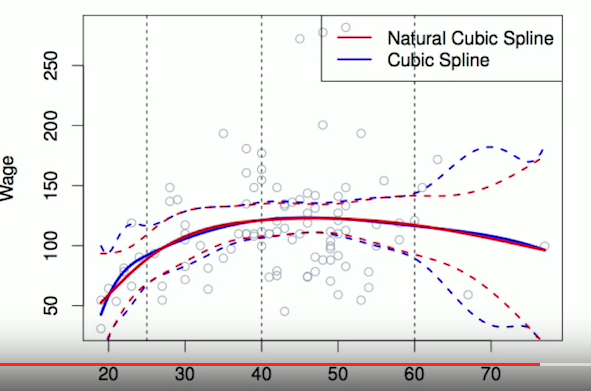
\includegraphics[width=.5\textwidth]{cubic_splines.png}
\caption{It shows the difference between Natural Cubic Spline and Cubic Spline.}
\end{figure}
Knot placement
\begin{itemize}
\item One strategy is to decide $K$, the number of knots, and then palce them at appropriate quantiles of the observed $X$.
\item A cubic spline with $K$ knots has $K+4$ paramters or degree of freedom.
\item A natural spline with $K$ knots has $K$ degrees of freedom.
\end{itemize}
Smoothing Splines\\
Consider fitting a smooth function to some data
\[
  \min_{g\in \mathcal{S}}=\sum_{i=1}^n(y_i-g(x_i))^2+\lambda\int g''(t)^2dt
\]
\begin{itemize}
\item The first term is RSS, and tries to make $g(x)$ match data at each $x_i$.
\item The second term is a \emph{roughness penalty} and controls how wiggly $g(x)$ is. It is modulated by the tuning parameter $\lambda\geq 0$.
  \begin{itemize}
    \item The smaller $\lambda$, the more wiggly the function, eventually interpolating $y_i$ when $\lambda=0$.
    \item As $\lambda \rightarrow \infty$, the function $g(x)$ becomes linear.
    \item The solution is a natural cubic spline, with a knot at every unique value of $x_i$. The roughness peanlty still controls the roughness via $\lambda$.
  \end{itemize}
\end{itemize}
Some details about Smoothing Spline
\begin{itemize}
  \item Smoothing splines avoid the knot-selection issue, leaving single $\lambda$ to be chosen.
  \item The vector of $n$ fitted values can be written as $\hat{g}_\lambda=\mathbf{S}_\lambda \mathbf{y}$, where $\mathbf{S}_\lambda$ is a $n\times n$ matrix (determined by the $x_i$ and $\lambda$)
\item The effective degrees of feedom are given by 
\[
  df_\lambda=\sum_{i=1}^n\{\mathbf{S}_\lambda\}_{ii}.
\]
\item We can specify $df$ rather than $\lambda$.
\end{itemize}
Local Regression\\
With a sliding weight function, we fit separate linear fits over the range of $X$ by weighed least squares.\\[1mm]
Generalized Additive Models\\
Allows for flexible non-linearities in several variables, but retain the additive structure of linear models.
\[
  y_i=\beta_0+f_1(x_{ij})+f_2(x_{i2})+\dots+f_p(x_{ip}) + \epsilon_i
\]
GAMs for classification
\[
  \log\bigg(\frac{p(X)}{1-p(X)}\bigg)=\beta_0+f_1(X_1)+f_2(X_2)+\dots+f_p(X_p).
\]
\section{Tree-based methods}
\begin{itemize}
\item It involves stratifying or segmenting the predictor space into a number of simple regions.
\item Since the set of splitting rules used to segment the predictor psace can be summarized in a tree, these types of approaches are known as decision-tree methods.
\end{itemize}
\subsection{Terminology for Trees}
\begin{itemize}
\item In keeping with the tree analogy, the regions $R_1,R_2, R_3$ are known as terminal nodes.
\item Decision trees are typically drawn upside down, in the sense that the leaves are at the bottom of the tree.
\item The points along the tree where the predictor space is split are referred to as internal nodes
\end{itemize}
\subsection{Tree-building process}
\begin{itemize}
\item In theory, the regions could have any shape. However, we choose to divide the predictor space into high-dimensional rectangles, or boxes, for simplicity and for ease of interpretation of the resulting predictive model
\item The goal is to find boxes $R_1,\dots,R_J$ that minimize the RSS, given by
\[
  \sum_{j=1}^J\sum_{i\in R_j} (y_i-\hat{y}_{R_j})^2.  
\]
where $\hat{y}_{R_j}$ is the mean response for the training observations within the $j$th box, which is also one of the terminal leaves.
\item It is computationally infeasible to consider every possible partition of the feature space into $J$ boxes
\item For this reason, we take a top-down, greedy approach that is know as recursive binary splitting
\item The approach is top-down because it begins at the top of the tree and then succesively splits the predictor space; each split is indicated via two new branches further down on the tree
\item It is greedy because at each step of the tree-building process, the best split is made at that particular step, rather than looking ahead and picking a split that will lead to a better tree in some future step.
\item We predict the response for a given test observation using the mean of the training observations in the region to which that test observation belongs.
\end{itemize}
\subsection{Pruning a tree}
\begin{itemize}
\item Grow a very large tree $T_0$, and then prune it back in order to obtain a subtree.
\item cost complexity pruning --- also known as weakest link pruning is used to do this.
\item We consider a sequence of trees indexed by a nonnegative tuning parameter $\alpha$. For each value of $\alpha$ there corresponds a subtree $T\subset T_0$ such that 
  \[
    \sum_{m=1}^{|T|}\sum_{i:x_i\in R_m}(y_i-\hat{y}_{R_m})^2+\alpha|T|
  \]
  is as small as possible. Here $|T|$ indicates that the number of terminal nodes of the tree $T$, $Rm$ is the rectangle (i.e. the subseet of predictor space) corresonding to the $m$th terminal node, and $\hat{y}_{R_m}$ is the mean of the training observations in $R_m$. The formulation is similar to the Lasso.
\item The tuning paramter $\alpha$ controls a trade-off between the subtree's complexity and its fit to the training data.
\item We select an optimal value $\hat{\alpha}$ using cross-validation.
\item We then return to the full data set and obtain the subtree corresponding to $\hat{\alpha}$.
\end{itemize}
\subsection{Classification Trees}
\begin{itemize}
  \item Very similar to a regression tree, except that it is used to predict a qualitative response rather than a quantitative one.
  \item For a classification tree, we predict that each observation belongs to the most commonly occurring class of training observations in the region to which it belongs.
  \item In the classification setting, RSS cannot be used as a criterion for making the binary splits
  \item A natural alternative to RSS is the classification error rate. this is simply the fraction fo the training observations in that region that do not belong to the most common class:
\[
  E=1-\max_k(\hat{p}_{mk}).
\]
Here $\hat{p}_{mk}$ represents the proportion of training observation in the $m$th region that are from the $k$th class
\item Classification error is not sufficiently sensitive for tree-growing, and in practice two other measures are preferable.
\item The Gini index is defined by
\[
  G=\sum_{k=1}^K\hat{p}_{mk}(1-\hat{p}_{mk})  
\]
a measure of total variance across the $K$ classes. The Gini index takes on a small value if all of the $\hat{p}_{mk}$'s are close to zero or one
\item For this reason the Gini index is referred to as a measure of node purity --- a small value indicates that a node contains predominantly observations from a single class.
\item An alternative to the Gini index is cross-entropy, given by 
  \[
    D=-\sum_{k=1}^K\hat{p}_{mk}\log\hat{p}_{mk}.
  \]
\item It turns out that the Gini index and the cross-entropy are very similar numerically.
\end{itemize}
\subsection{Bagging}
\begin{itemize}
  \item Bootstrap aggregation or bagging, is a general-purpose procedure for reducing the variance of a statistical learning method.
  \item Recall that given a set of $n$ indepedent observations $Z_1,\dots,Z_n$, each with variance $\sigma^2$, the variance of the mean $\bar{Z}$ of the observations is given by $\sigma^2/n$.
  \item In other words, averaging set of observations reduces variance.
  \item We generate $B$ different bootstrapped trainnig data sets. We then train our method on the $b$th bootstrapped training set in order to get $\hat{f}^{*b}(x)$, the prediction at a point $x$. We then average all the prediction to obatin
\[
  \hat{f}_{bag}(x)={1\over B}\sum_{b=1}^B\hat{f}^{*b}(x)
\]
\item For classification trees: for each test observation, we record the class predicted by each of the $B$ trees, and take a majority vote: the overall prediction is the most common occurring class among the $B$ predictions.
  \end{itemize}
Out-of-Bag Error Estimation
\begin{itemize}
  \item There is a very straightforward way to estimate the test error of a bagged model.
  \item On can show that on average, each bagged tree makes use of around two-thirds of the observations.
  \item The remaining one-third of the observations not used to fit a given bagged tree are referred to as the out-of-bag (OOB) observations
  \item We can predict the response for the $i$th observation using each of the trees in which that observations was OOB. This will yield around $B/3$ predictions for the $i$th observation which we average.
  \item This estimate is essentially the LOO cross-validation erro for bagging, if $B$ is large.
\end{itemize}
Random Forests
\begin{itemize}
\item RF provide an improvement over bagged trees by way of a small tweak that decorrelates the trees. This reduces the variance when we average the trees.
\item As in bagging, we build a number of decision trees on bootstrapped training samples.
\item But when building these decision trees, each time a split in a tree is considered, a random selection of $m$ predictors is chosen as split candidates from the full set of $p$ predictors. The split is allowed to use only one of those $m$ predictors.
\item A fresh selection of $m$ predictors is taken at each split, and typicaly we choose $m\approx \sqrt{p}$ --- that is, the number of predictors considered at each split is approxmately equal to the square root of the total number of predictors.
\end{itemize}
\subsection{Boosting}
Boosting for decision trees works in a similar way as bagging, except that trees are grown sequentially: each tree is grown using information from preivsouly grown trees.
\begin{figure}
[h!]
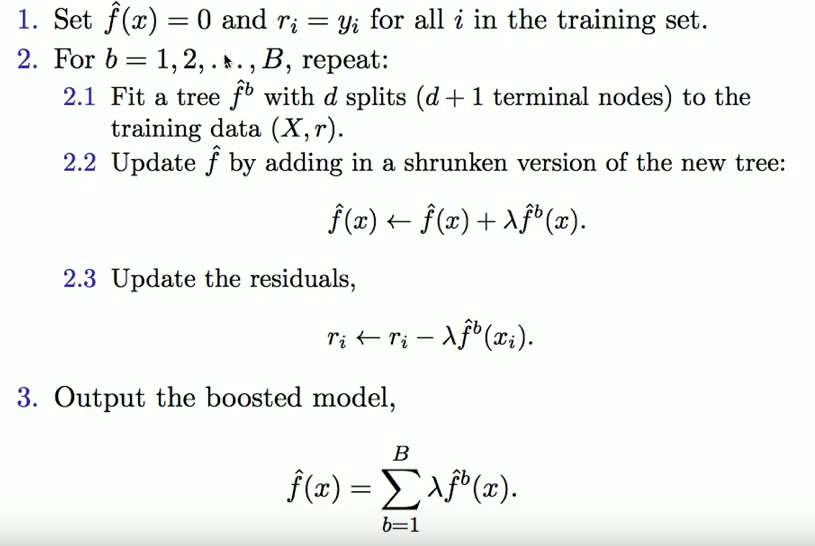
\includegraphics[width=.6\textwidth]{boosting.png}
\caption{Boosting algorithm.}
\end{figure}\\
Idea behind
\begin{itemize}
\item Unlike fitting a single large decision tree to the data, which amounts to fitting the data hard and potentially overfitting, the boosting approach instead learns slowly.
\item Given the current model, we fit a decision tree to the residuals from the model. We then add this new decision tree into the fitted function in order to update the residuals.
\item Each of these trees can be rather small, with just a few terminal nodes, determined by the parameter $d$ in the algorithm.
\item By fitting small trees to the residuals, we slowly improve $\hat{f}$ in areas where it does not perform well. The shrinkage parameter $\lambda$ slows the process down even further, allowing more and different shaped trees to attack the residuals.
\end{itemize}
\section{Support Vector Machines}
We try and find a plane that separates the classes in feature space.\\
If we cannot, we get creative in two ways:
\begin{itemize}
\item We soften what we eman by ``separates'', and 
\item We enrich and enlarge the feature space so that separation is possible.
\end{itemize}
What is a Hyperplane?
\begin{itemize}
  \item A hyperplane in $p$ dimension is a flat affine subspace of dimension $p-1$.
\item In general the equation for a hyperplane has the form
  \[
  \beta_0+\beta_1X_1+\beta_2X_2+\dots+\beta_pX_p=0.
  \]
\item In $p=2$ dimensions a hyperplane is is a line
\item If $\beta_0=0$, then the hyperplane goes through the origin, otherwise not.
\item The vector $\beta=(\beta_1,\beta_2,\dots\beta_p)$ is called the normal vector --- it points in a direction orthogonal to the surface of a hyperplane.
\end{itemize}
Maximal Margin Classifier\\
Among all separating hyperplaens, find the one that makes the biggest gap or margin between the two classes.\\
Constrained optimization problem
\[
  \underset{\beta_0,\beta_1,\dots,\beta_p}{\operatorname{maximize}} M
\]
subject to $\sum_{j=1}^p \beta_j^2 = 1,$, $y_i(\beta_0+\beta_1x_{i1}+\dots+\beta_px_{ip})\geq M$  for all $i=1,\dots,N$.
The data is separable when $N<p$, such as the genome data. When non-separable, the support vector classifier maximizes a soft margin.\\[1mm]
Support Vector Classifier\\
$\underset{\beta_0,\beta_1,\dots,\beta_p,\epsilon_1,\dots\epsilon_n}{\operatorname{maximize}} M$ subject to $\sum_{j=1}^p \beta_j^2=1$,  $y_i(\beta_0+\beta_1x_{i1}+\dots+\beta_px_{ip})\geq M(1-\epsilon_i)$, $\epsilon\geq 0$, $\sum_{i=1}^n \epsilon_i \leq C$.\\
$\epsilon$ is a slack which allows for some errors inside the margins, $C$ is a regularization parameter, which is a budget of $\epsilon$. Increasing $C$ makes the margin ``softer,'' so that the orientation of the separating hyperplane is influenced by more points. \\
\textbf{Note.} Lasso and Ridge Regression and SVMs treat the samples equally, so they should be standardized beforehand.\\[1mm]
Feature Expansion
\begin{itemize}
  \item Enlarge the space of features by including transformations; e.g. $X_1^2, X_1^3, X_1X_2, X_1X_2^2,\dots$. Hence go from a $p$ dimensional space to a $M>p$ dimensional space.
  \item Fit a support-vector classifier in teh enlarged space.
  \item This results in non-linear decision boudaries in the original space.
\item For example, suppose we use ($X_1,X_2,X_1^2,X_2^2,X_1 X_2$) instead of just ($X_1,X_2$). Then the decision boudary would be of the form
  \[
  \beta_0+ \beta_1 X_1+\beta_2 X_2+\beta_3 X_1^2+\beta_4 X_2^2+\beta_5 X_1 X_2=0
  \]
  \end{itemize}

This leads to nonlinear decision boudaries in the original space (Cubic Polynomials). It is linear in the new variable space, which results in a linear boundary in the high dimensional space. But nonlinear in the original space. In the lower dimensional space, however, these are conic sections of a quadratic polynomial.
Inner products and support vectors
\begin{itemize}
\item The linear support vector classifier can be represented as 
  \[
    f(x)=\beta_0+\sum_{i=1}^n \alpha_i\langle x,x_i\rangle \text{  --- \emph{n parameters}}.
  \]
\item To estimate the parameters $\alpha_1,\dots,\alpha_n$ and $\beta_0$, all we need are the $n \choose 2$ inner products $\langle x_i, x_{i'}$ between all pairs of training observations.
\item It turns out that most of the $\hat{\alpha}_i$ can be zero:
\[
  f(x)=\beta_0+\sum_{i\in \mathcal{S}}\hat{\alpha}_i\langle x,x_i\rangle ,
\]
where $\mathcal{S}$ is the support set of indices $i$ such that $\hat{\alpha}_i>0$. It is a sparsity in the data space.
\end{itemize}
Kernels and Support Vector Machines
\begin{itemize}
  \item If we can compute inner-products between observations, we can fit a SV classifier. It can be quite abstract.
  \item Some special \emph{kernel functions} can do this for us. E.g.
\[
  K(x_i,x_{i'})=\bigg(1+\sum_{j=1}^p x_{ij}x_{i'j}   \bigg)^d
\]
computes the inner-products needed for $d$ dimensional polynomials --- ${p+d\choose d}$ basis functions.
\item The solution has the form
  \[
    f(x)=\beta_0+\sum_{i\in\mathcal{S}}\hat{\alpha}_i K(x,x_i).
  \]
  Radial Kernel\\
  \[
    K(x_i,x_{i'})=\exp(-\gamma \sum_{j=1}^p(x_{ij}-x_{i'j})^2),
  \]
  It has an implicit feature space, and is very high dimesnional, It controls variance by squashing down most dimensions severely.\\[1mm]
More than 2 classes\\
\textbf{OVA}: One versus All. Fit $K$ different 2-class SVM classifiers $\hat{f}_k(x)$, k=1,\dots,K; each class versus the rest. Classify $x^*$ to the class for which $\hat{f}_k(x^*)$ is largest.\\
\textbf{OVO}: One versus One. Fit all $K \choose 2$ pairwise classifiers $\hat{f}_{k\ell}(x)$. Classify $x^*$ to the class that wins the most pairwise competitions.
\end{itemize}
Support Vector Machines vs Logistic Regression\\
With $f(X)=\beta_0+\beta_1X_1+\dots+\beta_pX_p$ can rephrase support vector classifier optimization as
\[
\underset{\beta_0,\beta_1,\dots,\beta_p}{\operatorname{minimize}}\bigg( \max 0.1-y_i f(x_i)]+\lambda\sum_{j=1}^p\beta_j^2\bigg)
\]
\begin{figure}
[h!]
\centering
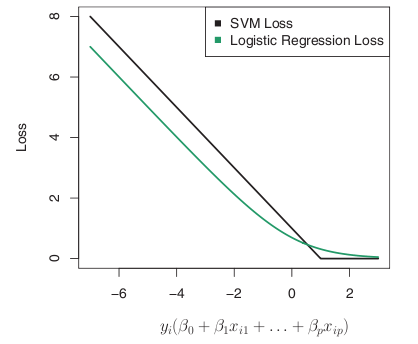
\includegraphics[width=.4\textwidth]{svm.png}
\caption{SVMs vs Logistic Regression.}
\end{figure}
This has the form loss plus penalty. This loss is known as the hinge loss, which is very similar to ``loss'' in logistic regression (negative log-likelihood).\\
Which one to use
\begin{itemize}
\item When clases are nearly separable, SVM and LDA do better than LR.
\item When not, LR (with ridge penalty) and SVM perform similarly.
\item If you wish to etimate probabilities, LR is the choice.
\item For nonlinear boundaries, kernel SVMs are popular. Can use kernels with LR and LDA as well, but computations are more expensive.
\end{itemize}
\section{Unsupervised learning}
\subsection{PCA}
The principal component direction $\phi_1,\phi_2,\phi_3\dots$ are the ordered sequence of right singular vectors of the matrix $\mathbf{X}$, and the variances of the components are ${1\over n} $ times the squares of the singular values. There are at most $\min(n-1,p)$ principal components.\par
Hyperplane on PCA and linear regression. For linear regression, we measure the distance from the label $y$ to the point in the hyperplane. By contrast, PCA finds the shortest distance from the data points to the hyperplane, and the distance is perpendicular to the hyperplane. In other words, we find a hyperplane that passes through the middle of the data points, We compute the distance from the data points to the hyperplane and sum the sqauress of the distance. We want the hyperplane that gets closest to the data.\par
Scaling of the variables matters --- If the varaibles are in different units, scaling each to have standard deviation equal to one is recommended.\\
\begin{itemize}
  \item The first principal component of a set of features $X_1,X_2,\dots,X_p$ is the normalized lienar combinaton of the features 
\[
  Z_1=\phi_{11}X_1+\phi_{21}X_2+\dots+\phi_{p1}X_p    
\]
that has the largest variance. By normalized, we mean that $\sum_{j=1}^p\phi_{j1}^2=1$.
\item We refer to the elements $\phi_{11},\dots,\phi_{p1}$ as the loadings of the first principal component; together, the loadings make up the principal component loading vector, $\phi_1=(\phi_{11} \phi_{21} \dots \phi_p1)^\top$.
\item We constrain the loadings so that theri sum of squares is equal to one, since otherwise setting these elements to be arbitrarily large in absolute value could result in an arbitrarily large variance.
  \end{itemize}
Proportion Variance Explained
\begin{itemize}
  \item To understand the strength of each PCA component, we are interested in knowing the proportion of variance explained (PVE) by each one.
  \item The total variance present in data set (assuming that the varaibles have been centered to have mean zero) is defined as
\[
  \sum_{j=1}^p\operatorname{Var}(X_j)=\sum_{j=1}^p{1\over n}\sum_{i=1}^n x^2_{ij}    
\]
and the variance explained by the $m$th principal component is 
\[
  \operatorname{Var}(Z_m)={1\over n}\sum_{i=1}^n z_{im}^2
\]
\item It can be shown that $\sum_{j=1}^p\operatorname{Var}(X_j)=\sum_{m=1}^M\operatorname{Var}(Z_m)$, with $M=\min(n-1,p)$.
\item the PVE of the $m$th principal component is given by the positive quantity between 0 and 1
\[
  \frac{\sum_{i=1}^n z_{im}^2}{\sum_{j=1}^p\sum_{j=1}^n x_{ij}^2} 
\]
\item The PVEs sum to one. We sometimes display the cumulative PVEs.
\end{itemize}
To select the number of components, we could use cross-validation to find the number of components used in regression. We cannot use the cross-validation directly due to the lack of reponse.
\subsection{Clustering}
K-means
\begin{itemize}
  \item The idea behind K-means clustering is a good clustering is one for which the within-cluster variation is as small as possible.
  \item The within-cluster variation for cluster $C_k$ is a measure $WCV(C_k)$ of the amount by which the observations within a cluster differ from each other.
  \item We want to solve the problem
\begin{align}
\underset{C1,\dots,C_k}{\operatorname{minimize}}\bigg\{\sum_{k=1}^K WCV(C_k)\bigg\}
  =\underset{C_1,\dots,C_K}{\operatorname{minimize}}\bigg\{\sum_{k=1}^K {1\over |C_k|}\sum_{i,i'\in C_k}\sum_{j=1}^p (x_{ij}-x_{i' j})^2 \bigg\}.
\end{align}
\item The algorithm is guaranteed to decrease the value of the objective at each step. 
  \[
    {1\over |C_k|}\sum_{i,i'\in C_k}\sum^p_{j=1}(X_{ij}-x_{i'j})^2=2\sum_{i\in C_k}\sum_{j=1}^p(x_{ij}-\bar{x}_{kj})^2.
  \]
  where $\bar{x}_{kj}={1\over |C_k|}\sum_{i\in C_k x_{ij}}$ is the mean for feature $j$ in cluster $C_k$. However, it is not guaranteed to give the global minimum.
\end{itemize}
In hierarchical clustering, we do not know in advance how many clusters we want; in fact, we end up with a tree-like visual representation of the observations, called a dendrogram, that allows us to view at once the clusterings obtained for each possible number of clusters, from 1 to $n$.\\
In case of hierarchical clustering,
\begin{itemize}
\item What dissimilarity measure should be used
\item What type of linkage should be used
\end{itemize}
Some engineering can also be done to select the samples. In the breast cancer microarray example, they select 500 intrinsic genes out of 8000 genes, which have the smallest within/between variation. The intrinsic genes varies a lot between women but little within women.
\end{document}
